\documentclass[1p]{elsarticle_modified}
%\bibliographystyle{elsarticle-num}

%\usepackage[colorlinks]{hyperref}
%\usepackage{abbrmath_seonhwa} %\Abb, \Ascr, \Acal ,\Abf, \Afrak
\usepackage{amsfonts}
\usepackage{amssymb}
\usepackage{amsmath}
\usepackage{amsthm}
\usepackage{scalefnt}
\usepackage{amsbsy}
\usepackage{kotex}
\usepackage{caption}
\usepackage{subfig}
\usepackage{color}
\usepackage{graphicx}
\usepackage{xcolor} %% white, black, red, green, blue, cyan, magenta, yellow
\usepackage{float}
\usepackage{setspace}
\usepackage{hyperref}

\usepackage{tikz}
\usetikzlibrary{arrows}

\usepackage{multirow}
\usepackage{array} % fixed length table
\usepackage{hhline}

%%%%%%%%%%%%%%%%%%%%%
\makeatletter
\renewcommand*\env@matrix[1][\arraystretch]{%
	\edef\arraystretch{#1}%
	\hskip -\arraycolsep
	\let\@ifnextchar\new@ifnextchar
	\array{*\c@MaxMatrixCols c}}
\makeatother %https://tex.stackexchange.com/questions/14071/how-can-i-increase-the-line-spacing-in-a-matrix
%%%%%%%%%%%%%%%

\usepackage[normalem]{ulem}

\newcommand{\msout}[1]{\ifmmode\text{\sout{\ensuremath{#1}}}\else\sout{#1}\fi}
%SOURCE: \msout is \stkout macro in https://tex.stackexchange.com/questions/20609/strikeout-in-math-mode

\newcommand{\cancel}[1]{
	\ifmmode
	{\color{red}\msout{#1}}
	\else
	{\color{red}\sout{#1}}
	\fi
}

\newcommand{\add}[1]{
	{\color{blue}\uwave{#1}}
}

\newcommand{\replace}[2]{
	\ifmmode
	{\color{red}\msout{#1}}{\color{blue}\uwave{#2}}
	\else
	{\color{red}\sout{#1}}{\color{blue}\uwave{#2}}
	\fi
}

\newcommand{\Sol}{\mathcal{S}} %segment
\newcommand{\D}{D} %diagram
\newcommand{\A}{\mathcal{A}} %arc


%%%%%%%%%%%%%%%%%%%%%%%%%%%%%5 test

\def\sl{\operatorname{\textup{SL}}(2,\Cbb)}
\def\psl{\operatorname{\textup{PSL}}(2,\Cbb)}
\def\quan{\mkern 1mu \triangleright \mkern 1mu}

\theoremstyle{definition}
\newtheorem{thm}{Theorem}[section]
\newtheorem{prop}[thm]{Proposition}
\newtheorem{lem}[thm]{Lemma}
\newtheorem{ques}[thm]{Question}
\newtheorem{cor}[thm]{Corollary}
\newtheorem{defn}[thm]{Definition}
\newtheorem{exam}[thm]{Example}
\newtheorem{rmk}[thm]{Remark}
\newtheorem{alg}[thm]{Algorithm}

\newcommand{\I}{\sqrt{-1}}
\begin{document}

%\begin{frontmatter}
%
%\title{Boundary parabolic representations of knots up to 8 crossings}
%
%%% Group authors per affiliation:
%\author{Yunhi Cho} 
%\address{Department of Mathematics, University of Seoul, Seoul, Korea}
%\ead{yhcho@uos.ac.kr}
%
%
%\author{Seonhwa Kim} %\fnref{s_kim}}
%\address{Center for Geometry and Physics, Institute for Basic Science, Pohang, 37673, Korea}
%\ead{ryeona17@ibs.re.kr}
%
%\author{Hyuk Kim}
%\address{Department of Mathematical Sciences, Seoul National University, Seoul 08826, Korea}
%\ead{hyukkim@snu.ac.kr}
%
%\author{Seokbeom Yoon}
%\address{Department of Mathematical Sciences, Seoul National University, Seoul, 08826,  Korea}
%\ead{sbyoon15@snu.ac.kr}
%
%\begin{abstract}
%We find all boundary parabolic representation of knots up to 8 crossings.
%
%\end{abstract}
%\begin{keyword}
%    \MSC[2010] 57M25 
%\end{keyword}
%
%\end{frontmatter}

%\linenumbers
%\tableofcontents
%
\newcommand\colored[1]{\textcolor{white}{\rule[-0.35ex]{0.8em}{1.4ex}}\kern-0.8em\color{red} #1}%
%\newcommand\colored[1]{\textcolor{white}{ #1}\kern-2.17ex	\textcolor{white}{ #1}\kern-1.81ex	\textcolor{white}{ #1}\kern-2.15ex\color{red}#1	}

{\Large $\underline{12a_{1240}~(K12a_{1240})}$}

\setlength{\tabcolsep}{10pt}
\renewcommand{\arraystretch}{1.6}
\vspace{1cm}\begin{tabular}{m{100pt}>{\centering\arraybackslash}m{274pt}}
\multirow{5}{120pt}{
	\centering
	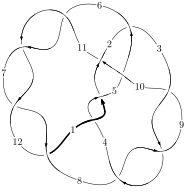
\includegraphics[width=112pt]{../../../GIT/diagram.site/Diagrams/png/2041_12a_1240.png}\\
\ \ \ A knot diagram\footnotemark}&
\allowdisplaybreaks
\textbf{Linearized knot diagam} \\
\cline{2-2}
 &
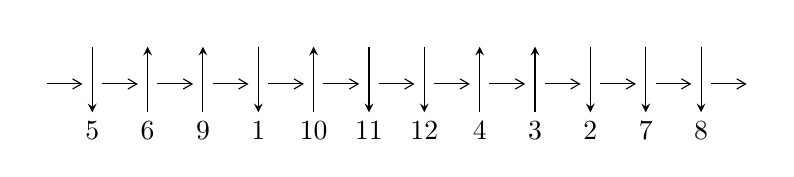
\begin{tikzpicture}[x=20pt, y=17pt]
	% nodes
	\node (C0) at (0, 0) {};
	\node (C1) at (1, 0) {};
	\node (C1U) at (1, +1) {};
	\node (C1D) at (1, -1) {5};

	\node (C2) at (2, 0) {};
	\node (C2U) at (2, +1) {};
	\node (C2D) at (2, -1) {6};

	\node (C3) at (3, 0) {};
	\node (C3U) at (3, +1) {};
	\node (C3D) at (3, -1) {9};

	\node (C4) at (4, 0) {};
	\node (C4U) at (4, +1) {};
	\node (C4D) at (4, -1) {1};

	\node (C5) at (5, 0) {};
	\node (C5U) at (5, +1) {};
	\node (C5D) at (5, -1) {10};

	\node (C6) at (6, 0) {};
	\node (C6U) at (6, +1) {};
	\node (C6D) at (6, -1) {11};

	\node (C7) at (7, 0) {};
	\node (C7U) at (7, +1) {};
	\node (C7D) at (7, -1) {12};

	\node (C8) at (8, 0) {};
	\node (C8U) at (8, +1) {};
	\node (C8D) at (8, -1) {4};

	\node (C9) at (9, 0) {};
	\node (C9U) at (9, +1) {};
	\node (C9D) at (9, -1) {3};

	\node (C10) at (10, 0) {};
	\node (C10U) at (10, +1) {};
	\node (C10D) at (10, -1) {2};

	\node (C11) at (11, 0) {};
	\node (C11U) at (11, +1) {};
	\node (C11D) at (11, -1) {7};

	\node (C12) at (12, 0) {};
	\node (C12U) at (12, +1) {};
	\node (C12D) at (12, -1) {8};
	\node (C13) at (13, 0) {};

	% arrows
	\draw[->,>={angle 60}]
	(C0) edge (C1) (C1) edge (C2) (C2) edge (C3) (C3) edge (C4) (C4) edge (C5) (C5) edge (C6) (C6) edge (C7) (C7) edge (C8) (C8) edge (C9) (C9) edge (C10) (C10) edge (C11) (C11) edge (C12) (C12) edge (C13) ;	\draw[->,>=stealth]
	(C1U) edge (C1D) (C2D) edge (C2U) (C3D) edge (C3U) (C4U) edge (C4D) (C5D) edge (C5U) (C6U) edge (C6D) (C7U) edge (C7D) (C8D) edge (C8U) (C9D) edge (C9U) (C10U) edge (C10D) (C11U) edge (C11D) (C12U) edge (C12D) ;
	\end{tikzpicture} \\
\hhline{~~} \\& 
\textbf{Solving Sequence} \\ \cline{2-2} 
 &
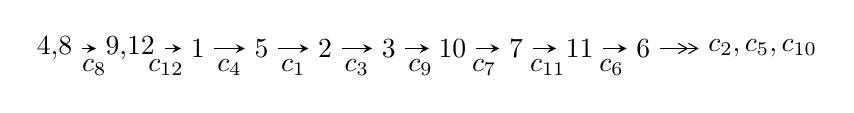
\begin{tikzpicture}[x=23pt, y=7pt]
	% node
	\node (A0) at (-1/8, 0) {4,8};
	\node (A1) at (17/16, 0) {9,12};
	\node (A2) at (17/8, 0) {1};
	\node (A3) at (25/8, 0) {5};
	\node (A4) at (33/8, 0) {2};
	\node (A5) at (41/8, 0) {3};
	\node (A6) at (49/8, 0) {10};
	\node (A7) at (57/8, 0) {7};
	\node (A8) at (65/8, 0) {11};
	\node (A9) at (73/8, 0) {6};
	\node (C1) at (1/2, -1) {$c_{8}$};
	\node (C2) at (13/8, -1) {$c_{12}$};
	\node (C3) at (21/8, -1) {$c_{4}$};
	\node (C4) at (29/8, -1) {$c_{1}$};
	\node (C5) at (37/8, -1) {$c_{3}$};
	\node (C6) at (45/8, -1) {$c_{9}$};
	\node (C7) at (53/8, -1) {$c_{7}$};
	\node (C8) at (61/8, -1) {$c_{11}$};
	\node (C9) at (69/8, -1) {$c_{6}$};
	\node (A10) at (11, 0) {$c_{2},c_{5},c_{10}$};

	% edge
	\draw[->,>=stealth]	
	(A0) edge (A1) (A1) edge (A2) (A2) edge (A3) (A3) edge (A4) (A4) edge (A5) (A5) edge (A6) (A6) edge (A7) (A7) edge (A8) (A8) edge (A9) ;
	\draw[->>,>={angle 60}]	
	(A9) edge (A10);
\end{tikzpicture} \\ 

\end{tabular} \\

\footnotetext{
The image of knot diagram is generated by the software ``\textbf{Draw programme}" developed by Andrew Bartholomew(\url{http://www.layer8.co.uk/maths/draw/index.htm\#Running-draw}), where we modified some parts for our purpose(\url{https://github.com/CATsTAILs/LinksPainter}).
}\phantom \\ \newline 
\centering \textbf{Ideals for irreducible components\footnotemark of $X_{\text{par}}$} 
 
\begin{align*}
I^u_{1}&=\langle 
4.60256\times10^{102} u^{64}+5.40064\times10^{102} u^{63}+\cdots+8.11475\times10^{103} b+1.59562\times10^{105},\\
\phantom{I^u_{1}}&\phantom{= \langle  }-7.53145\times10^{104} u^{64}+2.70697\times10^{104} u^{63}+\cdots+1.40385\times10^{106} a+3.91291\times10^{107},\\
\phantom{I^u_{1}}&\phantom{= \langle  }u^{65}+u^{64}+\cdots+354 u+173\rangle \\
I^u_{2}&=\langle 
u^{15}+8 u^{13}+u^{12}+23 u^{11}+6 u^{10}+26 u^9+12 u^8+4 u^7+8 u^6-9 u^5- u^4-2 u^3-2 u^2+b- u-1,\\
\phantom{I^u_{2}}&\phantom{= \langle  }- u^{16}+u^{15}+\cdots+a+1,\\
\phantom{I^u_{2}}&\phantom{= \langle  }u^{17}+10 u^{15}+40 u^{13}- u^{12}+80 u^{11}-7 u^{10}+80 u^9-18 u^8+31 u^7-21 u^6-4 u^5-11 u^4-5 u^3-3 u^2-2 u-1\rangle \\
\\
\end{align*}
\raggedright * 2 irreducible components of $\dim_{\mathbb{C}}=0$, with total 82 representations.\\
\footnotetext{All coefficients of polynomials are rational numbers. But the coefficients are sometimes approximated in decimal forms when there is not enough margin.}
\newpage
\renewcommand{\arraystretch}{1}
\centering \section*{I. $I^u_{1}= \langle 4.60\times10^{102} u^{64}+5.40\times10^{102} u^{63}+\cdots+8.11\times10^{103} b+1.60\times10^{105},\;-7.53\times10^{104} u^{64}+2.71\times10^{104} u^{63}+\cdots+1.40\times10^{106} a+3.91\times10^{107},\;u^{65}+u^{64}+\cdots+354 u+173 \rangle$}
\flushleft \textbf{(i) Arc colorings}\\
\begin{tabular}{m{7pt} m{180pt} m{7pt} m{180pt} }
\flushright $a_{4}=$&$\begin{pmatrix}0\\u\end{pmatrix}$ \\
\flushright $a_{8}=$&$\begin{pmatrix}1\\0\end{pmatrix}$ \\
\flushright $a_{9}=$&$\begin{pmatrix}1\\- u^2\end{pmatrix}$ \\
\flushright $a_{12}=$&$\begin{pmatrix}0.0536485 u^{64}-0.0192824 u^{63}+\cdots+13.4066 u-27.8726\\-0.0567184 u^{64}-0.0665534 u^{63}+\cdots-38.2451 u-19.6632\end{pmatrix}$ \\
\flushright $a_{1}=$&$\begin{pmatrix}0.110367 u^{64}+0.0472710 u^{63}+\cdots+51.6516 u-8.20942\\-0.0567184 u^{64}-0.0665534 u^{63}+\cdots-38.2451 u-19.6632\end{pmatrix}$ \\
\flushright $a_{5}=$&$\begin{pmatrix}0.0429065 u^{64}-0.00292175 u^{63}+\cdots+21.3658 u-11.3738\\-0.0125258 u^{64}-0.0125001 u^{63}+\cdots-10.2360 u-7.41086\end{pmatrix}$ \\
\flushright $a_{2}=$&$\begin{pmatrix}-0.0400474 u^{64}-0.000625365 u^{63}+\cdots-4.46978 u+16.5675\\0.00594570 u^{64}+0.0205051 u^{63}+\cdots+15.4488 u+6.51593\end{pmatrix}$ \\
\flushright $a_{3}=$&$\begin{pmatrix}- u\\u^3+u\end{pmatrix}$ \\
\flushright $a_{10}=$&$\begin{pmatrix}u^2+1\\- u^4-2 u^2\end{pmatrix}$ \\
\flushright $a_{7}=$&$\begin{pmatrix}0.0399289 u^{64}+0.0211829 u^{63}+\cdots+33.3413 u+0.333312\\-0.00290844 u^{64}-0.00912864 u^{63}+\cdots-5.74412 u-4.59512\end{pmatrix}$ \\
\flushright $a_{11}=$&$\begin{pmatrix}-0.0230777 u^{64}-0.0466096 u^{63}+\cdots-13.8268 u-24.0009\\-0.0279384 u^{64}-0.0319295 u^{63}+\cdots-19.5314 u-12.5317\end{pmatrix}$ \\
\flushright $a_{6}=$&$\begin{pmatrix}0.0320474 u^{64}+0.00430410 u^{63}+\cdots+17.5224 u-7.47526\\0.0150469 u^{64}+0.0130919 u^{63}+\cdots+1.71790 u-0.984422\end{pmatrix}$\\&\end{tabular}
\flushleft \textbf{(ii) Obstruction class $= -1$}\\~\\
\flushleft \textbf{(iii) Cusp Shapes $= 0.103545 u^{64}-0.0564918 u^{63}+\cdots+57.0917 u-87.3956$}\\~\\
\newpage\renewcommand{\arraystretch}{1}
\flushleft \textbf{(iv) u-Polynomials at the component}\newline \\
\begin{tabular}{m{50pt}|m{274pt}}
Crossings & \hspace{64pt}u-Polynomials at each crossing \\
\hline $$\begin{aligned}c_{1},c_{4}\end{aligned}$$&$\begin{aligned}
&u^{65}-34 u^{63}+\cdots+25 u-1
\end{aligned}$\\
\hline $$\begin{aligned}c_{2}\end{aligned}$$&$\begin{aligned}
&u^{65}-5 u^{64}+\cdots-1840 u-529
\end{aligned}$\\
\hline $$\begin{aligned}c_{3},c_{8},c_{9}\end{aligned}$$&$\begin{aligned}
&u^{65}+u^{64}+\cdots+354 u+173
\end{aligned}$\\
\hline $$\begin{aligned}c_{5}\end{aligned}$$&$\begin{aligned}
&u^{65}+2 u^{64}+\cdots+784 u+131
\end{aligned}$\\
\hline $$\begin{aligned}c_{6},c_{7},c_{11}\\c_{12}\end{aligned}$$&$\begin{aligned}
&u^{65}- u^{64}+\cdots+16 u+1
\end{aligned}$\\
\hline $$\begin{aligned}c_{10}\end{aligned}$$&$\begin{aligned}
&u^{65}+5 u^{64}+\cdots+1163 u-215
\end{aligned}$\\
\hline
\end{tabular}\\~\\
\newpage\renewcommand{\arraystretch}{1}
\flushleft \textbf{(v) Riley Polynomials at the component}\newline \\
\begin{tabular}{m{50pt}|m{274pt}}
Crossings & \hspace{64pt}Riley Polynomials at each crossing \\
\hline $$\begin{aligned}c_{1},c_{4}\end{aligned}$$&$\begin{aligned}
&y^{65}-68 y^{64}+\cdots-201 y-1
\end{aligned}$\\
\hline $$\begin{aligned}c_{2}\end{aligned}$$&$\begin{aligned}
&y^{65}+27 y^{64}+\cdots-5322798 y-279841
\end{aligned}$\\
\hline $$\begin{aligned}c_{3},c_{8},c_{9}\end{aligned}$$&$\begin{aligned}
&y^{65}+77 y^{64}+\cdots-683978 y-29929
\end{aligned}$\\
\hline $$\begin{aligned}c_{5}\end{aligned}$$&$\begin{aligned}
&y^{65}+20 y^{64}+\cdots-271428 y-17161
\end{aligned}$\\
\hline $$\begin{aligned}c_{6},c_{7},c_{11}\\c_{12}\end{aligned}$$&$\begin{aligned}
&y^{65}-87 y^{64}+\cdots-500 y-1
\end{aligned}$\\
\hline $$\begin{aligned}c_{10}\end{aligned}$$&$\begin{aligned}
&y^{65}-25 y^{64}+\cdots+3288859 y-46225
\end{aligned}$\\
\hline
\end{tabular}\\~\\
\newpage\flushleft \textbf{(vi) Complex Volumes and Cusp Shapes}
$$\begin{array}{c|c|c}  
\text{Solutions to }I^u_{1}& \I (\text{vol} + \sqrt{-1}CS) & \text{Cusp shape}\\
 \hline 
\begin{aligned}
u &= \phantom{-}0.726071 + 0.758126 I \\
a &= -0.324975 - 0.706814 I \\
b &= -0.979305 + 0.369172 I\end{aligned}
 & -5.63744 + 7.47497 I & \phantom{-0.000000 } 0 \\ \hline\begin{aligned}
u &= \phantom{-}0.726071 - 0.758126 I \\
a &= -0.324975 + 0.706814 I \\
b &= -0.979305 - 0.369172 I\end{aligned}
 & -5.63744 - 7.47497 I & \phantom{-0.000000 } 0 \\ \hline\begin{aligned}
u &= \phantom{-}0.975827 + 0.494607 I \\
a &= -0.107308 + 0.453272 I \\
b &= \phantom{-}0.934240 + 0.048674 I\end{aligned}
 & -4.60698 - 1.82196 I & \phantom{-0.000000 } 0 \\ \hline\begin{aligned}
u &= \phantom{-}0.975827 - 0.494607 I \\
a &= -0.107308 - 0.453272 I \\
b &= \phantom{-}0.934240 - 0.048674 I\end{aligned}
 & -4.60698 + 1.82196 I & \phantom{-0.000000 } 0 \\ \hline\begin{aligned}
u &= \phantom{-}0.543682 + 0.626807 I \\
a &= -0.567121 - 1.246980 I \\
b &= -1.72542 + 0.11080 I\end{aligned}
 & -14.1457 + 2.3448 I & -11.61428 - 2.93633 I \\ \hline\begin{aligned}
u &= \phantom{-}0.543682 - 0.626807 I \\
a &= -0.567121 + 1.246980 I \\
b &= -1.72542 - 0.11080 I\end{aligned}
 & -14.1457 - 2.3448 I & -11.61428 + 2.93633 I \\ \hline\begin{aligned}
u &= -0.117879 + 1.166460 I \\
a &= -1.79246 + 0.68241 I \\
b &= -1.387970 + 0.003546 I\end{aligned}
 & -6.36326 - 2.20018 I & \phantom{-0.000000 } 0 \\ \hline\begin{aligned}
u &= -0.117879 - 1.166460 I \\
a &= -1.79246 - 0.68241 I \\
b &= -1.387970 - 0.003546 I\end{aligned}
 & -6.36326 + 2.20018 I & \phantom{-0.000000 } 0 \\ \hline\begin{aligned}
u &= \phantom{-}0.088335 + 0.787639 I \\
a &= \phantom{-}0.631221 + 0.409079 I \\
b &= \phantom{-}0.365744 - 0.340357 I\end{aligned}
 & -0.71879 + 1.22446 I & -2.81178 - 5.97989 I \\ \hline\begin{aligned}
u &= \phantom{-}0.088335 - 0.787639 I \\
a &= \phantom{-}0.631221 - 0.409079 I \\
b &= \phantom{-}0.365744 + 0.340357 I\end{aligned}
 & -0.71879 - 1.22446 I & -2.81178 + 5.97989 I\\
 \hline 
 \end{array}$$\newpage$$\begin{array}{c|c|c}  
\text{Solutions to }I^u_{1}& \I (\text{vol} + \sqrt{-1}CS) & \text{Cusp shape}\\
 \hline 
\begin{aligned}
u &= \phantom{-}0.447830 + 0.608444 I \\
a &= -1.60044 - 0.14443 I \\
b &= -1.59034 - 0.09596 I\end{aligned}
 & -8.81586 - 2.32152 I & -8.51550 - 4.26961 I \\ \hline\begin{aligned}
u &= \phantom{-}0.447830 - 0.608444 I \\
a &= -1.60044 + 0.14443 I \\
b &= -1.59034 + 0.09596 I\end{aligned}
 & -8.81586 + 2.32152 I & -8.51550 + 4.26961 I \\ \hline\begin{aligned}
u &= \phantom{-}0.525484 + 0.504088 I \\
a &= \phantom{-}0.43025 + 2.02495 I \\
b &= \phantom{-}1.69411 + 0.00431 I\end{aligned}
 & -13.75730 + 1.38625 I & -12.86514 - 4.98182 I \\ \hline\begin{aligned}
u &= \phantom{-}0.525484 - 0.504088 I \\
a &= \phantom{-}0.43025 - 2.02495 I \\
b &= \phantom{-}1.69411 - 0.00431 I\end{aligned}
 & -13.75730 - 1.38625 I & -12.86514 + 4.98182 I \\ \hline\begin{aligned}
u &= -0.334819 + 0.628588 I \\
a &= -0.278152 - 0.888652 I \\
b &= \phantom{-}0.103555 + 0.660906 I\end{aligned}
 & -2.26471 - 4.03136 I & -5.94020 + 7.20403 I \\ \hline\begin{aligned}
u &= -0.334819 - 0.628588 I \\
a &= -0.278152 + 0.888652 I \\
b &= \phantom{-}0.103555 - 0.660906 I\end{aligned}
 & -2.26471 + 4.03136 I & -5.94020 - 7.20403 I \\ \hline\begin{aligned}
u &= -0.983839 + 0.840083 I \\
a &= \phantom{-}0.958856 - 0.844751 I \\
b &= \phantom{-}1.71710 + 0.09388 I\end{aligned}
 & -15.1766 - 9.3107 I & \phantom{-0.000000 } 0 \\ \hline\begin{aligned}
u &= -0.983839 - 0.840083 I \\
a &= \phantom{-}0.958856 + 0.844751 I \\
b &= \phantom{-}1.71710 - 0.09388 I\end{aligned}
 & -15.1766 + 9.3107 I & \phantom{-0.000000 } 0 \\ \hline\begin{aligned}
u &= \phantom{-}0.317310 + 0.626994 I \\
a &= \phantom{-}2.68952 + 0.91215 I \\
b &= \phantom{-}1.61060 - 0.07096 I\end{aligned}
 & -9.00930 + 4.95002 I & -7.74249 - 6.87275 I \\ \hline\begin{aligned}
u &= \phantom{-}0.317310 - 0.626994 I \\
a &= \phantom{-}2.68952 - 0.91215 I \\
b &= \phantom{-}1.61060 + 0.07096 I\end{aligned}
 & -9.00930 - 4.95002 I & -7.74249 + 6.87275 I\\
 \hline 
 \end{array}$$\newpage$$\begin{array}{c|c|c}  
\text{Solutions to }I^u_{1}& \I (\text{vol} + \sqrt{-1}CS) & \text{Cusp shape}\\
 \hline 
\begin{aligned}
u &= \phantom{-}0.177809 + 1.350850 I \\
a &= -0.357829 + 0.197902 I \\
b &= -0.017560 + 0.381554 I\end{aligned}
 & -4.20596 + 3.45721 I & \phantom{-0.000000 } 0 \\ \hline\begin{aligned}
u &= \phantom{-}0.177809 - 1.350850 I \\
a &= -0.357829 - 0.197902 I \\
b &= -0.017560 - 0.381554 I\end{aligned}
 & -4.20596 - 3.45721 I & \phantom{-0.000000 } 0 \\ \hline\begin{aligned}
u &= -0.401140 + 0.489673 I \\
a &= \phantom{-}1.45507 + 0.87862 I \\
b &= \phantom{-}0.0202678 + 0.0500323 I\end{aligned}
 & -1.70244 + 1.41602 I & -3.83791 + 4.34485 I \\ \hline\begin{aligned}
u &= -0.401140 - 0.489673 I \\
a &= \phantom{-}1.45507 - 0.87862 I \\
b &= \phantom{-}0.0202678 - 0.0500323 I\end{aligned}
 & -1.70244 - 1.41602 I & -3.83791 - 4.34485 I \\ \hline\begin{aligned}
u &= -1.261060 + 0.536996 I \\
a &= -0.741092 + 0.442516 I \\
b &= -1.70945 + 0.01249 I\end{aligned}
 & -14.0841 + 2.0654 I & \phantom{-0.000000 } 0 \\ \hline\begin{aligned}
u &= -1.261060 - 0.536996 I \\
a &= -0.741092 - 0.442516 I \\
b &= -1.70945 - 0.01249 I\end{aligned}
 & -14.0841 - 2.0654 I & \phantom{-0.000000 } 0 \\ \hline\begin{aligned}
u &= -0.134645 + 0.584405 I \\
a &= \phantom{-}0.197801 - 1.366820 I \\
b &= \phantom{-}0.927502 + 0.501106 I\end{aligned}
 & -4.67220 + 0.02550 I & -14.8497 + 0.6733 I \\ \hline\begin{aligned}
u &= -0.134645 - 0.584405 I \\
a &= \phantom{-}0.197801 + 1.366820 I \\
b &= \phantom{-}0.927502 - 0.501106 I\end{aligned}
 & -4.67220 - 0.02550 I & -14.8497 - 0.6733 I \\ \hline\begin{aligned}
u &= -0.413347 + 0.412272 I \\
a &= -1.49091 + 0.92346 I \\
b &= -0.707354 - 0.303831 I\end{aligned}
 & -1.02330 - 3.62936 I & -5.37000 + 9.36655 I \\ \hline\begin{aligned}
u &= -0.413347 - 0.412272 I \\
a &= -1.49091 - 0.92346 I \\
b &= -0.707354 + 0.303831 I\end{aligned}
 & -1.02330 + 3.62936 I & -5.37000 - 9.36655 I\\
 \hline 
 \end{array}$$\newpage$$\begin{array}{c|c|c}  
\text{Solutions to }I^u_{1}& \I (\text{vol} + \sqrt{-1}CS) & \text{Cusp shape}\\
 \hline 
\begin{aligned}
u &= -0.372758 + 0.426791 I \\
a &= \phantom{-}0.574567 - 0.058040 I \\
b &= \phantom{-}0.625825 - 0.291328 I\end{aligned}
 & -1.20365 + 0.84496 I & -6.02969 - 0.14737 I \\ \hline\begin{aligned}
u &= -0.372758 - 0.426791 I \\
a &= \phantom{-}0.574567 + 0.058040 I \\
b &= \phantom{-}0.625825 + 0.291328 I\end{aligned}
 & -1.20365 - 0.84496 I & -6.02969 + 0.14737 I \\ \hline\begin{aligned}
u &= -0.233988 + 0.506859 I \\
a &= -0.55207 + 2.38792 I \\
b &= -0.886599 - 0.003824 I\end{aligned}
 & -4.55371 - 1.42223 I & -13.6222 + 4.9294 I \\ \hline\begin{aligned}
u &= -0.233988 - 0.506859 I \\
a &= -0.55207 - 2.38792 I \\
b &= -0.886599 + 0.003824 I\end{aligned}
 & -4.55371 + 1.42223 I & -13.6222 - 4.9294 I \\ \hline\begin{aligned}
u &= -0.16373 + 1.44899 I \\
a &= -1.220880 + 0.298307 I \\
b &= -0.980392 + 0.272927 I\end{aligned}
 & -7.19630 - 1.13487 I & \phantom{-0.000000 } 0 \\ \hline\begin{aligned}
u &= -0.16373 - 1.44899 I \\
a &= -1.220880 - 0.298307 I \\
b &= -0.980392 - 0.272927 I\end{aligned}
 & -7.19630 + 1.13487 I & \phantom{-0.000000 } 0 \\ \hline\begin{aligned}
u &= \phantom{-}0.483700 + 0.237329 I \\
a &= \phantom{-}0.445616 + 0.385675 I \\
b &= -0.083539 - 0.423218 I\end{aligned}
 & \phantom{-}0.791769 + 1.065080 I & \phantom{-}2.72009 - 3.18149 I \\ \hline\begin{aligned}
u &= \phantom{-}0.483700 - 0.237329 I \\
a &= \phantom{-}0.445616 - 0.385675 I \\
b &= -0.083539 + 0.423218 I\end{aligned}
 & \phantom{-}0.791769 - 1.065080 I & \phantom{-}2.72009 + 3.18149 I \\ \hline\begin{aligned}
u &= -0.10831 + 1.47851 I \\
a &= \phantom{-}1.76451 - 0.09693 I \\
b &= \phantom{-}0.952847 + 0.203501 I\end{aligned}
 & -7.28087 - 5.40688 I & \phantom{-0.000000 } 0 \\ \hline\begin{aligned}
u &= -0.10831 - 1.47851 I \\
a &= \phantom{-}1.76451 + 0.09693 I \\
b &= \phantom{-}0.952847 - 0.203501 I\end{aligned}
 & -7.28087 + 5.40688 I & \phantom{-0.000000 } 0\\
 \hline 
 \end{array}$$\newpage$$\begin{array}{c|c|c}  
\text{Solutions to }I^u_{1}& \I (\text{vol} + \sqrt{-1}CS) & \text{Cusp shape}\\
 \hline 
\begin{aligned}
u &= -0.497221\phantom{ +0.000000I} \\
a &= -0.274816\phantom{ +0.000000I} \\
b &= \phantom{-}1.21610\phantom{ +0.000000I}\end{aligned}
 & -2.77118\phantom{ +0.000000I} & \phantom{-}1.37870\phantom{ +0.000000I} \\ \hline\begin{aligned}
u &= -0.05022 + 1.56060 I \\
a &= \phantom{-}1.22584 - 0.84884 I \\
b &= \phantom{-}0.893368 + 0.290820 I\end{aligned}
 & -11.64490 - 2.37865 I & \phantom{-0.000000 } 0 \\ \hline\begin{aligned}
u &= -0.05022 - 1.56060 I \\
a &= \phantom{-}1.22584 + 0.84884 I \\
b &= \phantom{-}0.893368 - 0.290820 I\end{aligned}
 & -11.64490 + 2.37865 I & \phantom{-0.000000 } 0 \\ \hline\begin{aligned}
u &= \phantom{-}0.15087 + 1.57314 I \\
a &= -2.17718 - 1.21481 I \\
b &= -1.69886 + 0.07549 I\end{aligned}
 & \phantom{-}18.6332 + 3.8056 I & \phantom{-0.000000 } 0 \\ \hline\begin{aligned}
u &= \phantom{-}0.15087 - 1.57314 I \\
a &= -2.17718 + 1.21481 I \\
b &= -1.69886 - 0.07549 I\end{aligned}
 & \phantom{-}18.6332 - 3.8056 I & \phantom{-0.000000 } 0 \\ \hline\begin{aligned}
u &= -0.08895 + 1.58719 I \\
a &= -0.128172 - 0.447048 I \\
b &= \phantom{-}0.041223 + 0.495260 I\end{aligned}
 & -9.03428 - 0.28268 I & \phantom{-0.000000 } 0 \\ \hline\begin{aligned}
u &= -0.08895 - 1.58719 I \\
a &= -0.128172 + 0.447048 I \\
b &= \phantom{-}0.041223 - 0.495260 I\end{aligned}
 & -9.03428 + 0.28268 I & \phantom{-0.000000 } 0 \\ \hline\begin{aligned}
u &= -0.02863 + 1.60404 I \\
a &= -1.029160 + 0.070588 I \\
b &= -0.974979 - 0.838184 I\end{aligned}
 & -12.36230 - 0.51802 I & \phantom{-0.000000 } 0 \\ \hline\begin{aligned}
u &= -0.02863 - 1.60404 I \\
a &= -1.029160 - 0.070588 I \\
b &= -0.974979 + 0.838184 I\end{aligned}
 & -12.36230 + 0.51802 I & \phantom{-0.000000 } 0 \\ \hline\begin{aligned}
u &= -0.08706 + 1.60503 I \\
a &= -0.173991 - 0.074369 I \\
b &= -0.141617 - 0.998457 I\end{aligned}
 & -9.99826 - 5.54560 I & \phantom{-0.000000 } 0\\
 \hline 
 \end{array}$$\newpage$$\begin{array}{c|c|c}  
\text{Solutions to }I^u_{1}& \I (\text{vol} + \sqrt{-1}CS) & \text{Cusp shape}\\
 \hline 
\begin{aligned}
u &= -0.08706 - 1.60503 I \\
a &= -0.173991 + 0.074369 I \\
b &= -0.141617 + 0.998457 I\end{aligned}
 & -9.99826 + 5.54560 I & \phantom{-0.000000 } 0 \\ \hline\begin{aligned}
u &= \phantom{-}0.08728 + 1.61094 I \\
a &= -2.73738 - 0.27305 I \\
b &= -1.71337 + 0.05252 I\end{aligned}
 & -16.8071 + 6.4261 I & \phantom{-0.000000 } 0 \\ \hline\begin{aligned}
u &= \phantom{-}0.08728 - 1.61094 I \\
a &= -2.73738 + 0.27305 I \\
b &= -1.71337 - 0.05252 I\end{aligned}
 & -16.8071 - 6.4261 I & \phantom{-0.000000 } 0 \\ \hline\begin{aligned}
u &= \phantom{-}0.16484 + 1.61723 I \\
a &= \phantom{-}1.93553 + 0.68337 I \\
b &= \phantom{-}1.78156 - 0.24078 I\end{aligned}
 & \phantom{-}17.6410 + 5.0053 I & \phantom{-0.000000 } 0 \\ \hline\begin{aligned}
u &= \phantom{-}0.16484 - 1.61723 I \\
a &= \phantom{-}1.93553 - 0.68337 I \\
b &= \phantom{-}1.78156 + 0.24078 I\end{aligned}
 & \phantom{-}17.6410 - 5.0053 I & \phantom{-0.000000 } 0 \\ \hline\begin{aligned}
u &= \phantom{-}0.20239 + 1.63940 I \\
a &= \phantom{-}1.181390 + 0.350848 I \\
b &= \phantom{-}1.078620 - 0.622811 I\end{aligned}
 & -13.7279 + 10.9139 I & \phantom{-0.000000 } 0 \\ \hline\begin{aligned}
u &= \phantom{-}0.20239 - 1.63940 I \\
a &= \phantom{-}1.181390 - 0.350848 I \\
b &= \phantom{-}1.078620 + 0.622811 I\end{aligned}
 & -13.7279 - 10.9139 I & \phantom{-0.000000 } 0 \\ \hline\begin{aligned}
u &= \phantom{-}0.10820 + 1.65060 I \\
a &= \phantom{-}2.27932 + 0.08486 I \\
b &= \phantom{-}1.72742 + 0.06163 I\end{aligned}
 & -16.9343 - 0.1738 I & \phantom{-0.000000 } 0 \\ \hline\begin{aligned}
u &= \phantom{-}0.10820 - 1.65060 I \\
a &= \phantom{-}2.27932 - 0.08486 I \\
b &= \phantom{-}1.72742 - 0.06163 I\end{aligned}
 & -16.9343 + 0.1738 I & \phantom{-0.000000 } 0 \\ \hline\begin{aligned}
u &= \phantom{-}0.26868 + 1.68165 I \\
a &= -0.897135 - 0.531965 I \\
b &= -0.951609 + 0.306784 I\end{aligned}
 & -12.11670 + 3.02699 I & \phantom{-0.000000 } 0\\
 \hline 
 \end{array}$$\newpage$$\begin{array}{c|c|c}  
\text{Solutions to }I^u_{1}& \I (\text{vol} + \sqrt{-1}CS) & \text{Cusp shape}\\
 \hline 
\begin{aligned}
u &= \phantom{-}0.26868 - 1.68165 I \\
a &= -0.897135 + 0.531965 I \\
b &= -0.951609 - 0.306784 I\end{aligned}
 & -12.11670 - 3.02699 I & \phantom{-0.000000 } 0 \\ \hline\begin{aligned}
u &= -0.30378 + 1.69326 I \\
a &= -1.89667 + 0.85876 I \\
b &= -1.74870 - 0.17461 I\end{aligned}
 & \phantom{-}15.9285 - 14.2148 I & \phantom{-0.000000 } 0 \\ \hline\begin{aligned}
u &= -0.30378 - 1.69326 I \\
a &= -1.89667 - 0.85876 I \\
b &= -1.74870 + 0.17461 I\end{aligned}
 & \phantom{-}15.9285 + 14.2148 I & \phantom{-0.000000 } 0 \\ \hline\begin{aligned}
u &= -0.43555 + 1.77362 I \\
a &= \phantom{-}1.73566 - 0.73698 I \\
b &= \phantom{-}1.71505 + 0.08053 I\end{aligned}
 & \phantom{-}17.8768 - 4.5753 I & \phantom{-0.000000 } 0 \\ \hline\begin{aligned}
u &= -0.43555 - 1.77362 I \\
a &= \phantom{-}1.73566 + 0.73698 I \\
b &= \phantom{-}1.71505 - 0.08053 I\end{aligned}
 & \phantom{-}17.8768 + 4.5753 I & \phantom{-0.000000 } 0\\
 \hline 
 \end{array}$$\newpage\newpage\renewcommand{\arraystretch}{1}
\centering \section*{II. $I^u_{2}= \langle u^{15}+8 u^{13}+\cdots+b-1,\;- u^{16}+u^{15}+\cdots+a+1,\;u^{17}+10 u^{15}+\cdots-2 u-1 \rangle$}
\flushleft \textbf{(i) Arc colorings}\\
\begin{tabular}{m{7pt} m{180pt} m{7pt} m{180pt} }
\flushright $a_{4}=$&$\begin{pmatrix}0\\u\end{pmatrix}$ \\
\flushright $a_{8}=$&$\begin{pmatrix}1\\0\end{pmatrix}$ \\
\flushright $a_{9}=$&$\begin{pmatrix}1\\- u^2\end{pmatrix}$ \\
\flushright $a_{12}=$&$\begin{pmatrix}u^{16}- u^{15}+\cdots- u-1\\- u^{15}-8 u^{13}+\cdots+u+1\end{pmatrix}$ \\
\flushright $a_{1}=$&$\begin{pmatrix}u^{16}+10 u^{14}+\cdots-2 u-2\\- u^{15}-8 u^{13}+\cdots+u+1\end{pmatrix}$ \\
\flushright $a_{5}=$&$\begin{pmatrix}- u^{16}-10 u^{14}+\cdots+u+2\\- u^{15}+u^{14}+\cdots+2 u^3+2 u\end{pmatrix}$ \\
\flushright $a_{2}=$&$\begin{pmatrix}- u^5-3 u^3-2 u\\u^{16}- u^{15}+\cdots- u^2+u\end{pmatrix}$ \\
\flushright $a_{3}=$&$\begin{pmatrix}- u\\u^3+u\end{pmatrix}$ \\
\flushright $a_{10}=$&$\begin{pmatrix}u^2+1\\- u^4-2 u^2\end{pmatrix}$ \\
\flushright $a_{7}=$&$\begin{pmatrix}u^{15}- u^{14}+\cdots+u^3-2 u\\u^{15}+9 u^{13}+\cdots-2 u-2\end{pmatrix}$ \\
\flushright $a_{11}=$&$\begin{pmatrix}- u^6-4 u^4-3 u^2+1\\u^{15}+8 u^{13}+\cdots- u^2- u\end{pmatrix}$ \\
\flushright $a_{6}=$&$\begin{pmatrix}- u^{16}-9 u^{14}+\cdots+3 u^2+1\\- u^{15}+u^{14}+\cdots+2 u^3+u\end{pmatrix}$\\&\end{tabular}
\flushleft \textbf{(ii) Obstruction class $= 1$}\\~\\
\flushleft \textbf{(iii) Cusp Shapes $= - u^{16}-3 u^{15}-8 u^{14}-26 u^{13}-24 u^{12}-85 u^{11}-31 u^{10}-126 u^9-12 u^8-75 u^7+6 u^6+u^5+13 u^4+16 u^3+19 u^2+7 u-6$}\\~\\
\newpage\renewcommand{\arraystretch}{1}
\flushleft \textbf{(iv) u-Polynomials at the component}\newline \\
\begin{tabular}{m{50pt}|m{274pt}}
Crossings & \hspace{64pt}u-Polynomials at each crossing \\
\hline $$\begin{aligned}c_{1}\end{aligned}$$&$\begin{aligned}
&u^{17}+3 u^{16}+\cdots-3 u-1
\end{aligned}$\\
\hline $$\begin{aligned}c_{2}\end{aligned}$$&$\begin{aligned}
&u^{17}+3 u^{15}+\cdots+2 u-1
\end{aligned}$\\
\hline $$\begin{aligned}c_{3}\end{aligned}$$&$\begin{aligned}
&u^{17}+10 u^{15}+\cdots-2 u+1
\end{aligned}$\\
\hline $$\begin{aligned}c_{4}\end{aligned}$$&$\begin{aligned}
&u^{17}-3 u^{16}+\cdots-3 u+1
\end{aligned}$\\
\hline $$\begin{aligned}c_{5}\end{aligned}$$&$\begin{aligned}
&u^{17}+u^{16}+\cdots+2 u^3+1
\end{aligned}$\\
\hline $$\begin{aligned}c_{6},c_{7}\end{aligned}$$&$\begin{aligned}
&u^{17}-12 u^{15}+\cdots+2 u+1
\end{aligned}$\\
\hline $$\begin{aligned}c_{8},c_{9}\end{aligned}$$&$\begin{aligned}
&u^{17}+10 u^{15}+\cdots-2 u-1
\end{aligned}$\\
\hline $$\begin{aligned}c_{10}\end{aligned}$$&$\begin{aligned}
&u^{17}+2 u^{16}+\cdots-3 u-1
\end{aligned}$\\
\hline $$\begin{aligned}c_{11},c_{12}\end{aligned}$$&$\begin{aligned}
&u^{17}-12 u^{15}+\cdots+2 u-1
\end{aligned}$\\
\hline
\end{tabular}\\~\\
\newpage\renewcommand{\arraystretch}{1}
\flushleft \textbf{(v) Riley Polynomials at the component}\newline \\
\begin{tabular}{m{50pt}|m{274pt}}
Crossings & \hspace{64pt}Riley Polynomials at each crossing \\
\hline $$\begin{aligned}c_{1},c_{4}\end{aligned}$$&$\begin{aligned}
&y^{17}-17 y^{16}+\cdots+11 y-1
\end{aligned}$\\
\hline $$\begin{aligned}c_{2}\end{aligned}$$&$\begin{aligned}
&y^{17}+6 y^{16}+\cdots-6 y-1
\end{aligned}$\\
\hline $$\begin{aligned}c_{3},c_{8},c_{9}\end{aligned}$$&$\begin{aligned}
&y^{17}+20 y^{16}+\cdots-2 y-1
\end{aligned}$\\
\hline $$\begin{aligned}c_{5}\end{aligned}$$&$\begin{aligned}
&y^{17}+3 y^{16}+\cdots+6 y^2-1
\end{aligned}$\\
\hline $$\begin{aligned}c_{6},c_{7},c_{11}\\c_{12}\end{aligned}$$&$\begin{aligned}
&y^{17}-24 y^{16}+\cdots+16 y-1
\end{aligned}$\\
\hline $$\begin{aligned}c_{10}\end{aligned}$$&$\begin{aligned}
&y^{17}-6 y^{16}+\cdots+3 y-1
\end{aligned}$\\
\hline
\end{tabular}\\~\\
\newpage\flushleft \textbf{(vi) Complex Volumes and Cusp Shapes}
$$\begin{array}{c|c|c}  
\text{Solutions to }I^u_{2}& \I (\text{vol} + \sqrt{-1}CS) & \text{Cusp shape}\\
 \hline 
\begin{aligned}
u &= -0.139852 + 1.214420 I \\
a &= \phantom{-}1.287590 + 0.470581 I \\
b &= \phantom{-}1.52103 + 0.06882 I\end{aligned}
 & -11.11750 - 4.71969 I & -12.69339 + 3.70079 I \\ \hline\begin{aligned}
u &= -0.139852 - 1.214420 I \\
a &= \phantom{-}1.287590 - 0.470581 I \\
b &= \phantom{-}1.52103 - 0.06882 I\end{aligned}
 & -11.11750 + 4.71969 I & -12.69339 - 3.70079 I \\ \hline\begin{aligned}
u &= \phantom{-}0.770505\phantom{ +0.000000I} \\
a &= \phantom{-}0.356369\phantom{ +0.000000I} \\
b &= -1.71199\phantom{ +0.000000I}\end{aligned}
 & -13.5631\phantom{ +0.000000I} & -10.8690\phantom{ +0.000000I} \\ \hline\begin{aligned}
u &= -0.313732 + 0.658301 I \\
a &= -2.46686 - 0.50202 I \\
b &= -1.56317 + 0.07758 I\end{aligned}
 & -8.98775 + 3.06986 I & -11.77160 - 5.40163 I \\ \hline\begin{aligned}
u &= -0.313732 - 0.658301 I \\
a &= -2.46686 + 0.50202 I \\
b &= -1.56317 - 0.07758 I\end{aligned}
 & -8.98775 - 3.06986 I & -11.77160 + 5.40163 I \\ \hline\begin{aligned}
u &= \phantom{-}0.150767 + 1.264220 I \\
a &= -0.036312 + 0.695026 I \\
b &= -0.280089 + 0.210720 I\end{aligned}
 & -4.79179 + 3.71423 I & -13.1910 - 5.6524 I \\ \hline\begin{aligned}
u &= \phantom{-}0.150767 - 1.264220 I \\
a &= -0.036312 - 0.695026 I \\
b &= -0.280089 - 0.210720 I\end{aligned}
 & -4.79179 - 3.71423 I & -13.1910 + 5.6524 I \\ \hline\begin{aligned}
u &= -0.155556 + 1.352930 I \\
a &= -1.43538 + 0.81001 I \\
b &= -1.195950 + 0.186568 I\end{aligned}
 & -7.82356 - 2.21494 I & -13.60579 + 3.56873 I \\ \hline\begin{aligned}
u &= -0.155556 - 1.352930 I \\
a &= -1.43538 - 0.81001 I \\
b &= -1.195950 - 0.186568 I\end{aligned}
 & -7.82356 + 2.21494 I & -13.60579 - 3.56873 I \\ \hline\begin{aligned}
u &= \phantom{-}0.344357 + 0.507264 I \\
a &= \phantom{-}1.69631 - 0.60701 I \\
b &= \phantom{-}0.435868 + 0.235200 I\end{aligned}
 & -1.98177 - 1.91528 I & -11.51112 + 7.56473 I\\
 \hline 
 \end{array}$$\newpage$$\begin{array}{c|c|c}  
\text{Solutions to }I^u_{2}& \I (\text{vol} + \sqrt{-1}CS) & \text{Cusp shape}\\
 \hline 
\begin{aligned}
u &= \phantom{-}0.344357 - 0.507264 I \\
a &= \phantom{-}1.69631 + 0.60701 I \\
b &= \phantom{-}0.435868 - 0.235200 I\end{aligned}
 & -1.98177 + 1.91528 I & -11.51112 - 7.56473 I \\ \hline\begin{aligned}
u &= -0.413428 + 0.204442 I \\
a &= -1.37361 - 0.56067 I \\
b &= \phantom{-}0.983355 + 0.195981 I\end{aligned}
 & -3.72761 + 0.27179 I & -7.30557 - 0.70090 I \\ \hline\begin{aligned}
u &= -0.413428 - 0.204442 I \\
a &= -1.37361 + 0.56067 I \\
b &= \phantom{-}0.983355 - 0.195981 I\end{aligned}
 & -3.72761 - 0.27179 I & -7.30557 + 0.70090 I \\ \hline\begin{aligned}
u &= -0.06863 + 1.60082 I \\
a &= -0.854604 + 0.519619 I \\
b &= -0.759245 - 0.457661 I\end{aligned}
 & -10.71870 - 1.63142 I & -9.76522 + 0.61847 I \\ \hline\begin{aligned}
u &= -0.06863 - 1.60082 I \\
a &= -0.854604 - 0.519619 I \\
b &= -0.759245 + 0.457661 I\end{aligned}
 & -10.71870 + 1.63142 I & -9.76522 - 0.61847 I \\ \hline\begin{aligned}
u &= \phantom{-}0.21082 + 1.61302 I \\
a &= \phantom{-}2.00469 + 0.90354 I \\
b &= \phantom{-}1.71420 - 0.09994 I\end{aligned}
 & -19.7367 + 3.7909 I & -9.22182 - 1.00044 I \\ \hline\begin{aligned}
u &= \phantom{-}0.21082 - 1.61302 I \\
a &= \phantom{-}2.00469 - 0.90354 I \\
b &= \phantom{-}1.71420 + 0.09994 I\end{aligned}
 & -19.7367 - 3.7909 I & -9.22182 + 1.00044 I\\
 \hline 
 \end{array}$$\newpage
\newpage\renewcommand{\arraystretch}{1}
\centering \section*{ III. u-Polynomials}
\begin{tabular}{m{50pt}|m{274pt}}
Crossings & \hspace{64pt}u-Polynomials at each crossing \\
\hline $$\begin{aligned}c_{1}\end{aligned}$$&$\begin{aligned}
&(u^{17}+3 u^{16}+\cdots-3 u-1)(u^{65}-34 u^{63}+\cdots+25 u-1)
\end{aligned}$\\
\hline $$\begin{aligned}c_{2}\end{aligned}$$&$\begin{aligned}
&(u^{17}+3 u^{15}+\cdots+2 u-1)(u^{65}-5 u^{64}+\cdots-1840 u-529)
\end{aligned}$\\
\hline $$\begin{aligned}c_{3}\end{aligned}$$&$\begin{aligned}
&(u^{17}+10 u^{15}+\cdots-2 u+1)(u^{65}+u^{64}+\cdots+354 u+173)
\end{aligned}$\\
\hline $$\begin{aligned}c_{4}\end{aligned}$$&$\begin{aligned}
&(u^{17}-3 u^{16}+\cdots-3 u+1)(u^{65}-34 u^{63}+\cdots+25 u-1)
\end{aligned}$\\
\hline $$\begin{aligned}c_{5}\end{aligned}$$&$\begin{aligned}
&(u^{17}+u^{16}+\cdots+2 u^3+1)(u^{65}+2 u^{64}+\cdots+784 u+131)
\end{aligned}$\\
\hline $$\begin{aligned}c_{6},c_{7}\end{aligned}$$&$\begin{aligned}
&(u^{17}-12 u^{15}+\cdots+2 u+1)(u^{65}- u^{64}+\cdots+16 u+1)
\end{aligned}$\\
\hline $$\begin{aligned}c_{8},c_{9}\end{aligned}$$&$\begin{aligned}
&(u^{17}+10 u^{15}+\cdots-2 u-1)(u^{65}+u^{64}+\cdots+354 u+173)
\end{aligned}$\\
\hline $$\begin{aligned}c_{10}\end{aligned}$$&$\begin{aligned}
&(u^{17}+2 u^{16}+\cdots-3 u-1)(u^{65}+5 u^{64}+\cdots+1163 u-215)
\end{aligned}$\\
\hline $$\begin{aligned}c_{11},c_{12}\end{aligned}$$&$\begin{aligned}
&(u^{17}-12 u^{15}+\cdots+2 u-1)(u^{65}- u^{64}+\cdots+16 u+1)
\end{aligned}$\\
\hline
\end{tabular}\newpage\renewcommand{\arraystretch}{1}
\centering \section*{ IV. Riley Polynomials}
\begin{tabular}{m{50pt}|m{274pt}}
Crossings & \hspace{64pt}Riley Polynomials at each crossing \\
\hline $$\begin{aligned}c_{1},c_{4}\end{aligned}$$&$\begin{aligned}
&(y^{17}-17 y^{16}+\cdots+11 y-1)(y^{65}-68 y^{64}+\cdots-201 y-1)
\end{aligned}$\\
\hline $$\begin{aligned}c_{2}\end{aligned}$$&$\begin{aligned}
&(y^{17}+6 y^{16}+\cdots-6 y-1)(y^{65}+27 y^{64}+\cdots-5322798 y-279841)
\end{aligned}$\\
\hline $$\begin{aligned}c_{3},c_{8},c_{9}\end{aligned}$$&$\begin{aligned}
&(y^{17}+20 y^{16}+\cdots-2 y-1)(y^{65}+77 y^{64}+\cdots-683978 y-29929)
\end{aligned}$\\
\hline $$\begin{aligned}c_{5}\end{aligned}$$&$\begin{aligned}
&(y^{17}+3 y^{16}+\cdots+6 y^2-1)(y^{65}+20 y^{64}+\cdots-271428 y-17161)
\end{aligned}$\\
\hline $$\begin{aligned}c_{6},c_{7},c_{11}\\c_{12}\end{aligned}$$&$\begin{aligned}
&(y^{17}-24 y^{16}+\cdots+16 y-1)(y^{65}-87 y^{64}+\cdots-500 y-1)
\end{aligned}$\\
\hline $$\begin{aligned}c_{10}\end{aligned}$$&$\begin{aligned}
&(y^{17}-6 y^{16}+\cdots+3 y-1)(y^{65}-25 y^{64}+\cdots+3288859 y-46225)
\end{aligned}$\\
\hline
\end{tabular}
\vskip 2pc
\end{document}